% chap1.tex {Introductory Chapter}

\chapter{Introduction}

\section{Brief Overview of Deep Neural Networks}
Deep convolutional neural networks have seen an enormous amount of success on a wide
array of application, from scene interpretation to self-driving vehicles and art generation.
Natural language processing tasks are no exception to the range of problems
deep learning can solve, from sentiment analysis to language modeling. In this work, we
focus on using convolutional neural networks for text classification. Especifically,
we analyse how well modern neural networks models performed using moderately-sized scientific
abstract text datasets from multiple disciplines such as astro-physics and computer science.
The term modern in this context refers to neural models that use popular and recently
(re)discovered techniques to achieve state-of-the-art performance on most machine learning
benchmark datasets.

\section{Training a Neural Network}
A neural network is a function $f(\bm{x};\bm{\theta})$ that maps its input $\bm{x}$ to some response variable $y$. When we \textit{train} a
neural network, we \textit{learn} the model parameters, or weights, $\bm{\theta}$ that minimize some cost function $J(\bm{\theta})$.
For a regression task, where the model's output is a continuous variable, a common cost function is the \textbf{Mean Square Error}:
\[J(\theta) = \frac{1}{m}\sum_{i=1}^{m}(y_{i} - f(\bm{x}_{i};\bm{\theta}))^{2}\]

For categorical or discrete output variables found in e.g. classification tasks, we use the \textbf{Categorical Cross-Entropy}:

\[J(\bm{\theta}) = -\mathbb{E}_{\bm{x},y \sim \hat p_{data}} \log \textit{p}(y|\bm{x};\bm{\theta})\]

Given a \textit{training} set of observations $\bm{x}_i$ and their true labels $y_i$, we compute weights that minimize the cost, or error, via
maximum likelihood (ML) estimation:

\[\bm{\theta}_{ML} = \argmax_{\bm{\theta}} \sum_{i}^{m} \log P(y_{i}|\bm{x}_{i};\bm{\theta})\],

which one can see is the equivalent of computing the weights that \textbf{\textit{minimize}} the cross-entropy cost function.


%\section{Minimizing Non-Convex Functions: Gradiant-Based Learning}
%Convex functions are easy to optimize. Their global minimum is guaranteed and any local minimum is a global minimum. This means that when a
%procedure optimizes a convex function, its solution is truly optimal[CITE]. Said procedure is also guaranteed to converge from any initial point in parameter space[CITE].
%Due to the non-linearities associated with a neural network, the loss function to be minimized becomes non-convex.
%[Elaborate (Weight symmetry, model identifiability, etc)]

%Because of the non-convexitivity of neural network optimization, we usually rely on gradient-based methods. This involves iteratively \textit{moving},
%or updating, the values of our weights in the direction opposite of the cost function's gradient. These updates should be small, scaled by a
%\textit{learning rate}, and can make learning a lengthy process. Nonetheless, this method is effective and allows for learning of a good
%set of weights, although in practive it is rarely the optimal[CITE].

\section{Bias-Variance Tradeoff}
When learning a neural network's weights, we use a \textit{training set} so that we can later generalize
previously unseen data with high accuracy (or some other determined metric). That means that during training, we
obtain $\bm{\theta}_{ML}$ by minimizing $J_{train}(\bm{\theta})$, but we care about having low $J_{test}(\bm{\theta})$ i.e. low cost
on test data points.

\begin{figure}[h]
\caption{Visualization of overfitting. Training error decreases as epochs progress, eventually reaching zero.
Validation error starts increasing, indicating overfitting. The best model is shown at the dotted line, where
validation error reached its minimum.}
\centering
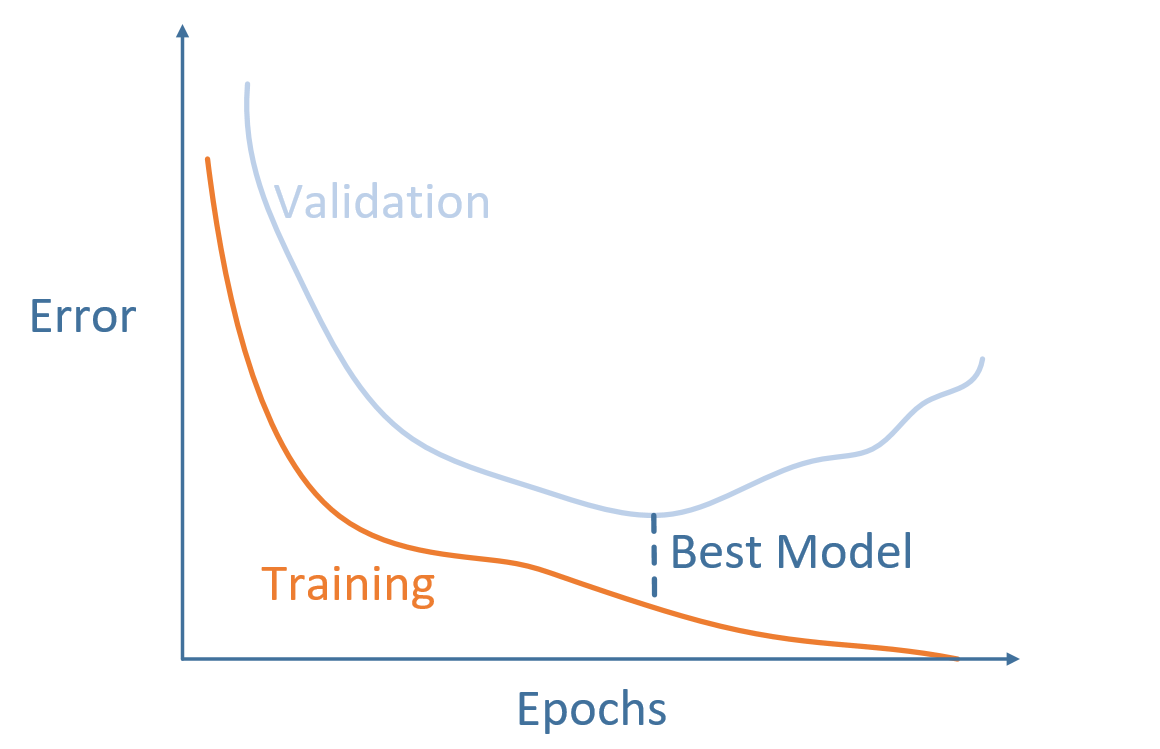
\includegraphics[width=0.5\textwidth]{OverfittingLossPlot.png}
\end{figure}

\textbf{Overfitting} occurs when a network is able to predict its training set extremely well i.e. very close to zero error, but fails to predict
unseen data points. This is because the network's weights have been extremely fine-tuned to \textit{fit} its training data, but do not fit or represent
data points outside of its training sample.
An overfitted model is said to have large \textbf{variance} and small \textbf{bias}. Conversely, underfitting occurs when the model fails to predict
the training set because it generalizes too harshly. This model is said to have large bias and small variance. When training a neural network,
we aim to find a balance between training cost and test cost, between overfitting and underfitting.

Because of the commonly large amount of weights in deep convolutional networks, it is easy to overfit even a moderate size training set[CITE].
It has been shown that when using a large enough dataset, neural networks are trained without overfitting, and thus generalize well
to new unseen data. Because of the abundance of data today, it is relatively easy to acquire large datasets, although this is not always the case.
In this work, we consider the case then the sizes of available datasets are moderately sized e.g. a tens of thousands.
We quantify the effects of regularization used to avoid overfitting in a neural network[REFER TO CHAPTER], and propose dataset augmentation techniques to
simulate a larger amount of available data.

\section{Weight Regularization}
One way to regularize a model to impose a constraint on its weights. By adding a penalty term to the cost function, we can shrink weights to avoid
them from blowing up in magnitude and overfitting to the training set. $\bm{L_2}$ regularization
adds the L2 norm of the weights to the cost function:

\[J(\bm{\theta}) = -\mathbb{E}_{\bm{x},y \sim \hat p_{data}} \log \textit{p}(y|\bm{x};\bm{\theta}) + \lambda \lVert \bm{\theta} \rVert_{2}\]

where $\lambda$ is the regularization control parameter. Higher values of $\lambda$ penalize more and a value of 0 leads to no regularization.

\subsection{Dropout}
A more recent and highly effective way to regularize a neural network is via \textbf{dropout}.
Dropout "deactivates" a neuron or unit with probability $p_{drop}$. We deactivate a unit
by setting its output to 0. This forces the network to not rely on certain
activations, since any unit will only be \textit{active} with probability $1-p_{drop}$[CITE].
